\documentclass{article}\usepackage[]{graphicx}\usepackage[]{color}
%% maxwidth is the original width if it is less than linewidth
%% otherwise use linewidth (to make sure the graphics do not exceed the margin)
\makeatletter
\def\maxwidth{ %
  \ifdim\Gin@nat@width>\linewidth
    \linewidth
  \else
    \Gin@nat@width
  \fi
}
\makeatother

\definecolor{fgcolor}{rgb}{0.345, 0.345, 0.345}
\newcommand{\hlnum}[1]{\textcolor[rgb]{0.686,0.059,0.569}{#1}}%
\newcommand{\hlstr}[1]{\textcolor[rgb]{0.192,0.494,0.8}{#1}}%
\newcommand{\hlcom}[1]{\textcolor[rgb]{0.678,0.584,0.686}{\textit{#1}}}%
\newcommand{\hlopt}[1]{\textcolor[rgb]{0,0,0}{#1}}%
\newcommand{\hlstd}[1]{\textcolor[rgb]{0.345,0.345,0.345}{#1}}%
\newcommand{\hlkwa}[1]{\textcolor[rgb]{0.161,0.373,0.58}{\textbf{#1}}}%
\newcommand{\hlkwb}[1]{\textcolor[rgb]{0.69,0.353,0.396}{#1}}%
\newcommand{\hlkwc}[1]{\textcolor[rgb]{0.333,0.667,0.333}{#1}}%
\newcommand{\hlkwd}[1]{\textcolor[rgb]{0.737,0.353,0.396}{\textbf{#1}}}%
\let\hlipl\hlkwb

\usepackage{framed}
\makeatletter
\newenvironment{kframe}{%
 \def\at@end@of@kframe{}%
 \ifinner\ifhmode%
  \def\at@end@of@kframe{\end{minipage}}%
  \begin{minipage}{\columnwidth}%
 \fi\fi%
 \def\FrameCommand##1{\hskip\@totalleftmargin \hskip-\fboxsep
 \colorbox{shadecolor}{##1}\hskip-\fboxsep
     % There is no \\@totalrightmargin, so:
     \hskip-\linewidth \hskip-\@totalleftmargin \hskip\columnwidth}%
 \MakeFramed {\advance\hsize-\width
   \@totalleftmargin\z@ \linewidth\hsize
   \@setminipage}}%
 {\par\unskip\endMakeFramed%
 \at@end@of@kframe}
\makeatother

\definecolor{shadecolor}{rgb}{.97, .97, .97}
\definecolor{messagecolor}{rgb}{0, 0, 0}
\definecolor{warningcolor}{rgb}{1, 0, 1}
\definecolor{errorcolor}{rgb}{1, 0, 0}
\newenvironment{knitrout}{}{} % an empty environment to be redefined in TeX

\usepackage{alltt}
\usepackage{natbib}



\IfFileExists{upquote.sty}{\usepackage{upquote}}{}
\begin{document}



\title{Using R to create a wordcloud from text in an ebook}
\author{Judy Minichelli}
\maketitle

\begin{abstract}
The article gives instructions on how to download text from an ebook and create a 
wordcloud in R.  A wordclouds is a data visualization that shows the most commonly used words in a large text dataset where size is proportional to frequency; words with the highest count appear larger and in bold.  The ebook used in this example
is "The Wonderful Wizard of Oz"

\end{abstract}

\textit{The Wonderful Wizard of Oz} was written by Frank Baum and published in 1900. It was the basis for the 1902 Broadway musical and the classic 1939 movie starring Judy Garland. 

\section{R Packages}

The following packages were installed and brought in with library: dplyr, gutenbergr, stringr, tidytext, tm, wordcloud.

    

The function below stores the result of the book text download in the dataframe "wizard". 

\begin{knitrout}
\definecolor{shadecolor}{rgb}{0.969, 0.969, 0.969}\color{fgcolor}\begin{kframe}
\begin{alltt}
\hlkwd{library}\hlstd{(gutenbergr)}
\hlstd{wizard}\hlkwb{<-}\hlkwd{gutenberg_download}\hlstd{(}\hlnum{55}\hlstd{)}
\end{alltt}
\end{kframe}
\end{knitrout}

This dataframe has two columns, one for each line in the book.

\noindent For this exercise, it is not necessary to exclude chapter headings and the first few pages of text; however, the procedures below will accomplish the task.  

\section{How to Clean Data}

\begin{knitrout}
\definecolor{shadecolor}{rgb}{0.969, 0.969, 0.969}\color{fgcolor}\begin{kframe}
\begin{alltt}
\hlkwd{library}\hlstd{(stringr)}
\end{alltt}


{\ttfamily\noindent\color{warningcolor}{\#\# Warning: package 'stringr' was built under R version 3.4.2}}\begin{alltt}
\hlkwd{library}\hlstd{(dplyr)}
\end{alltt}


{\ttfamily\noindent\color{warningcolor}{\#\# Warning: package 'dplyr' was built under R version 3.4.2}}

{\ttfamily\noindent\itshape\color{messagecolor}{\#\# \\\#\# Attaching package: 'dplyr'}}

{\ttfamily\noindent\itshape\color{messagecolor}{\#\# The following objects are masked from 'package:stats':\\\#\# \\\#\#\ \ \ \  filter, lag}}

{\ttfamily\noindent\itshape\color{messagecolor}{\#\# The following objects are masked from 'package:base':\\\#\# \\\#\#\ \ \ \  intersect, setdiff, setequal, union}}\begin{alltt}
\hlstd{wizard}\hlkwb{<-}\hlstd{wizard}\hlopt
  \hlkwd{filter}\hlstd{(}\hlopt{!}\hlkwd{str_detect}\hlstd{(wizard}\hlopt{$}\hlstd{text,}\hlstr{'^CHAPTER'}\hlstd{))}
\end{alltt}
\end{kframe}
\end{knitrout}

The actual text begins on line 10 and ends on 4721 so the wizard data frame can be redefined to exclude the first 9 lines. 

\begin{knitrout}
\definecolor{shadecolor}{rgb}{0.969, 0.969, 0.969}\color{fgcolor}\begin{kframe}
\begin{alltt}
\hlstd{wizard}\hlkwb{<-}\hlstd{wizard[}\hlnum{10}\hlopt{:}\hlnum{4721}\hlstd{,]}
\end{alltt}
\end{kframe}
\end{knitrout}

\section{The Wordcloud}
To make the wordcloud, break the text lines into words.

\begin{knitrout}
\definecolor{shadecolor}{rgb}{0.969, 0.969, 0.969}\color{fgcolor}\begin{kframe}
\begin{alltt}
\hlkwd{library}\hlstd{(tidytext)}
\hlstd{words_df}\hlkwb{<-}\hlstd{wizard}\hlopt
  \hlkwd{unnest_tokens}\hlstd{(word,text)}

\hlstd{words_df}
\end{alltt}
\begin{verbatim}
## # A tibble: 39,695 x 2
##    gutenberg_id         word
##           <int>        <chr>
##  1           55     contents
##  2           55 introduction
##  3           55            1
##  4           55          the
##  5           55      cyclone
##  6           55            2
##  7           55          the
##  8           55      council
##  9           55         with
## 10           55          the
## # ... with 39,685 more rows
\end{verbatim}
\end{kframe}
\end{knitrout}

Remove commonly used "generic" words from the data frame, for example articles, prepositions, and pronouns like "the", "after", and "you" from the data frame using the stop\_words command.

\begin{knitrout}
\definecolor{shadecolor}{rgb}{0.969, 0.969, 0.969}\color{fgcolor}\begin{kframe}
\begin{alltt}
\hlstd{words_df}\hlkwb{<-}\hlstd{words_df}\hlopt
  \hlkwd{filter}\hlstd{(}\hlopt{!}\hlstd{(word} \hlopt \hlstd{stop_words}\hlopt{$}\hlstd{word))}

\hlstd{words_df}
\end{alltt}
\begin{verbatim}
## # A tibble: 12,304 x 2
##    gutenberg_id         word
##           <int>        <chr>
##  1           55     contents
##  2           55 introduction
##  3           55            1
##  4           55      cyclone
##  5           55            2
##  6           55      council
##  7           55    munchkins
##  8           55            3
##  9           55      dorothy
## 10           55        saved
## # ... with 12,294 more rows
\end{verbatim}
\end{kframe}
\end{knitrout}

Calculate the frequencies of the remaining unique words.  

\begin{knitrout}
\definecolor{shadecolor}{rgb}{0.969, 0.969, 0.969}\color{fgcolor}\begin{kframe}
\begin{alltt}
\hlstd{word_freq}\hlkwb{<-}\hlstd{words_df}\hlopt
  \hlkwd{group_by}\hlstd{(word)}\hlopt
  \hlkwd{summarize}\hlstd{(}\hlkwc{count}\hlstd{=}\hlkwd{n}\hlstd{())}

\hlstd{word_freq}
\end{alltt}
\begin{verbatim}
## # A tibble: 2,507 x 2
##     word count
##    <chr> <int>
##  1     1     2
##  2    10     2
##  3    11     2
##  4    12     2
##  5    13     2
##  6    14     2
##  7    15     2
##  8    16     2
##  9    17     2
## 10    18     2
## # ... with 2,497 more rows
\end{verbatim}
\end{kframe}
\end{knitrout}

Generate the wordcloud. If there are too many or too few words, adjust "n" in "min.freq=n" to change the minimum number of occurances required for the word to appear in the wordcloud.  The number of colors used in the graphic can be changed by adjusting "n" in "colors=brewer.pal(n,'Dark2').  This helps further differentiate  the words used with higher frequency.  

\begin{knitrout}
\definecolor{shadecolor}{rgb}{0.969, 0.969, 0.969}\color{fgcolor}\begin{kframe}
\begin{alltt}
\hlkwd{library}\hlstd{(wordcloud)}
\hlkwd{library}\hlstd{(tm)}
\hlkwd{wordcloud}\hlstd{(word_freq}\hlopt{$}\hlstd{word,word_freq}\hlopt{$}\hlstd{count,}\hlkwc{min.freq}\hlstd{=}\hlnum{20}\hlstd{,}\hlkwc{colors}\hlstd{=}\hlkwd{brewer.pal}\hlstd{(}\hlnum{4}\hlstd{,}\hlstr{'Dark2'}\hlstd{))}
\end{alltt}
\end{kframe}
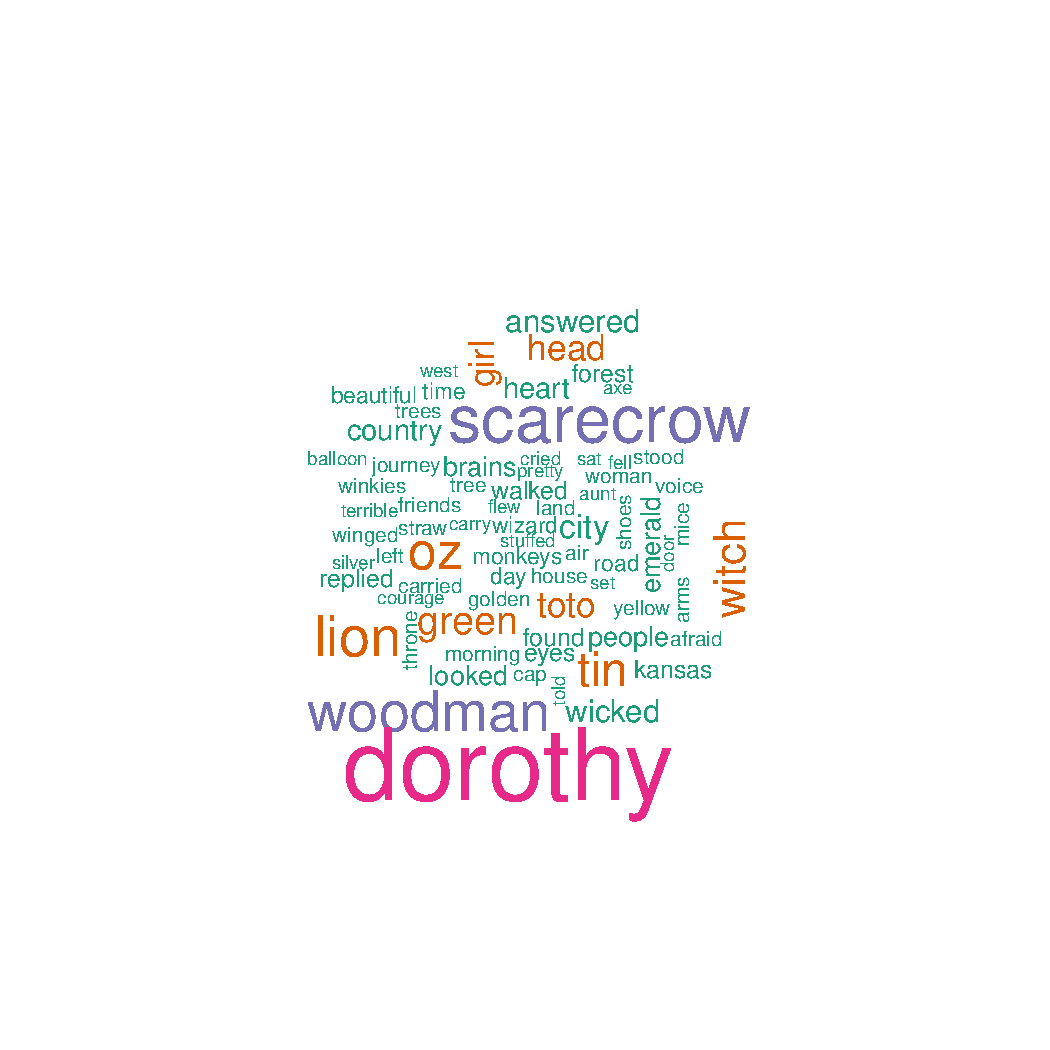
\includegraphics[width=\maxwidth]{figure/unnamed-chunk-8-1} 

\end{knitrout}

\bibliographystyle{apa}
\bibliography{article,wiz}
\nocite{*}

\end{document}
